\label{Konzept}
\chapter{Konzept}

\section{Grundkonzept}

	\begin{figure} %[hbtp]
		\centering
		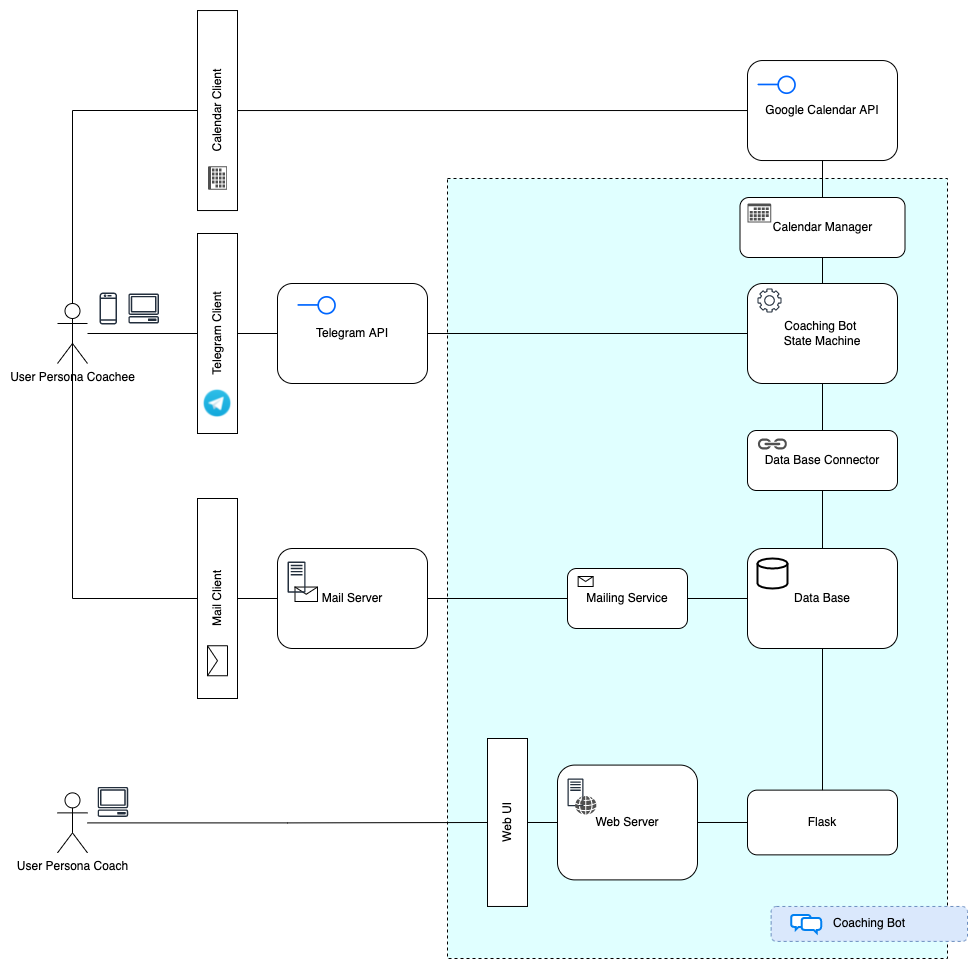
\includegraphics[width=1.0\textwidth]{images/220320_PA28464_Architecture.png}
		\caption{Konzeptionelle Architektur für das Projekt \emph{Der Coaching Bot}}
		\label{fig: architecture}
	\end{figure}

	Wie in Abbildung \ref{fig: architecture} skizziert, besteht der Kern des Bots auf einem endlichen Automaten (state machine), der Zustände vordefiniert und festlegt, wann sich welcher Nutzer in welchem Zustand befindet und von welchem in welchen Zustand er sich bewegen darf. An diesen Kern bindet sind als zentrales Steuerungselement des Bots alle anderen Systeme angebunden. Dazu gehören:
	\begin{enumerate}
		\item Die Datenbank zur Speicherung der Nutzerdaten
		\item Die Telegram API, über die die Kommunikation mit dem Telegram Client abgewickelt wird
		\item Die Google Calendar API, über die Events erstellt und versendet werden können
		\item Den Mail Server, über den E-Mails an den nutzer versendet werden können.
	\end{enumerate} 

	Der Nutzer interagiert mit dem ganzen System durch vier Kanäle - hier links ersichtlich:
	\begin{enumerate}
		\item Telegram Client: Kommunikation mit dem Bot
		\item Calendar Client: Erhalt, Annahme sowie Ablehnung der vereinbarten Termine
		\item Mail Client: Erhalten der Zusammenfassung und Bestätigung
		\item Web Browser: Übersicht über Anmeldungen und Terminkalender
	\end{enumerate}

	Der Bot wird von Benutzern (links oben) via einem der verfügbaren Telegram Clients angesprochen und reagiert auf die Eingabe entsprechend. So können verschieden Funktionen ausgelöst werden. Bspw. werden Antworten zurückgegeben, Informationen gespeichert oder es wird ein Vorschlag gemacht und an den Nutzer zurückgegeben. Der Bot soll mit mehreren Benutzern gleichzeitig sprechen können. Das wird ermöglicht, weil alle Reaktionen des Bots mit der Kennung des jeweiligen Nutzers verknüpft sind. So spricht der Bot den Nutzer mit Namen an oder kann sich daran erinnnern, welche Fragen schon beantwortet wurden und welche nicht. \\ \\

	Daneben gibt es einen zweite, sehr einfache Web-Applikation, die auf Flask basiert und eine Web-GUI zur Verfügung stellt, über die die gesammelten Informationen dargestellt werden können. So kann ein Coach (links unten) sich, nachdem Bewerber den Prozess beendet haben, alle gesammelten Informationen sowie vereinbarte Termine in einer einfachen Web-GUI ansehen.

\section{Zustände \& Konversationsfluss}

	Im folgenden Zustandsdiagramm ist der Konversationsfluss des Bots auf hohem Abstraktionsniveau, nämlich als endlicher Automat (state machine) abgebildet. Es wird deutlich, dass der Bot einem einfachen Skript folgt und komplizierte Loops vermieden werden. 
	\begin{figure} %[hbtp]
		\centering
		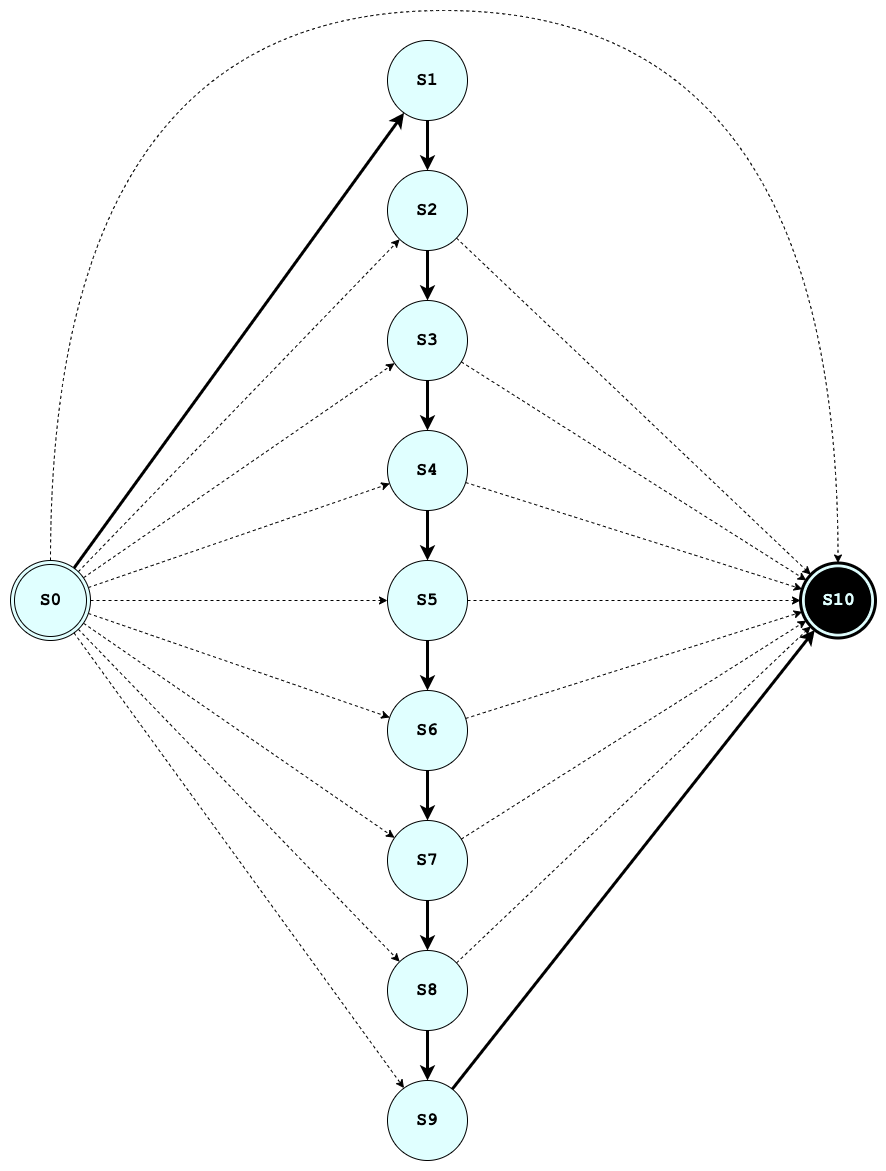
\includegraphics[width=1.0\textwidth]{images/220320_PA28464_State-Machine.png}
		\caption{Endlicher Automat des Konversationsflusses des Bots}
		\label{fig: state machine}
	\end{figure}

	Zustände:
	\begin{table} %[hbtp]
		\centering
		\begin{tabular}{l | l l l l}
			\textbf{Zustände} 	& \textbf{Beschreibung}\\
			\hline
			S0 					&		 START 			&		 Start: Applikation gestartet\\
			S1 					&		 BIO 			&		 Eingabemöglichkeit Biographie\\
			S2 					&		 GENDER 		&		 Eingabemöglichkeit Geschlecht\\
			S3 					&		 BIRTHDATE 		&		 Eingabemöglichkeit Geburtsdatum\\
			S4 					&		 EMAIL 			&		 Eingabemöglichkeit E-Mail Adresse\\
			S5 					&		 TELEPHONE 		&		 Eingabemöglichkeit Telefonnummer\\
			S6 					&		 LOCATION 		&		 Eingabemöglichkeit Ort\\
			S7 					&		 PHOTO 			&		 Eingabemöglichkeit Bild\\
			S8 					&		 SUMMARY 		&		 Zusammenfassung Daten\\
			S9 					&		 APPOINTMENT	&		 Terminvereinbarung \\
			S10 				&		 ENDE 			&		 Ende: Applikation beendet\\

		\end{tabular}
		\caption{Zustände des Konversationsflusses}
		\label{tab: states}
	\end{table}

	Der Haupt-Pfad ist hier fett eingezeichnet. Nebem diesem ist es aber auch möglich, dass der Nutzer nach einiger Zeit zum Bot zurück kommt und gerne an der Stelle weitermachen würde, wo er aufgehört hat. In diesem Fall, dient der Zustand \verb|S0| (START) als zentraler Einstiegspunkt. Hier wird analysiert, ob der Nutzer schon bekannt ist und falls ja, bis wohin er den Prozess bereits durchlaufen hat. Dann wird er dorthin weitergeleitet. Daher ist es möglich von START zu allen anderen Zuständen zu kommen, auch wenn das nicht die Regel ist. Hat der Nutzer den Prozess bereits abgeschlossen, so kann er sogar von S0 direkt in S10 (ENDE) landen und wird entsprechend benachrichtigt. Da dem Nutzer die Möglichkeit gegeben werden soll, den Prozess jederzeit zu beenden, ist es auch möglich, von jedem Zustand in \verb|S10| (ENDE) zu gelangen.
	
	\footnote{Der Konversationsfluss ist in einer sehr detaillierteren Ansicht verfügbar, in der der Unterschied zwischen dem hohen Abstraktionsniveau des Automaten und der Realität sichtbar wird. So lässt sich leicht erkennen, wo die Konversation beginnt und welche Zustände und Übergänge möglich sind: \url{https://github.com/mwel/coaching_bot/blob/main/thesis/images/220320_PA28464_Conversation_Flow.svg}} 